%!TEX root = main.tex
\section{Introduction}

%Exploring multidiemnsional dataset is hard
Visual data exploration is the \emph{de facto} first step in understanding a multi-dimensional dataset. This exploration serves a variety of purposes: identifying trends and patterns, spotting outliers and anomalies, and verifying hypotheses. However, as datasets grow in size and complexity, visual data exploration leads to several challenges for analyst. For example, to identify patterns that merit further investigation, an analyst may need to explore different subsets of the data, which grows exponentially in number of attributes. Generating and examining visualizations for this combinatorial space of data subsets is a major bottleneck in exploration.

%Drill-Down for exploration
One way of navigating this combinatorial space is to perform drill-downs on the lattice of data subsets. For example, a campaign manager interested in understanding the voting patterns across different demographics (say, race, gender, social class) using the 2016 US election exit polls\footnote{https://edition.cnn.com/election/2016/results/exit-polls} may first generate a bar chart for the entire population, where the x-axis shows the election candidates and the y-axis the percentage of votes for each of these candidates. This subset, refers to the overall population, is at the top of the lattice in Figure 1. They may then drill down to specific demographics of interest, say gender-based demographics, by generating bar charts for female voters (as shown in the Figure 1).

\begin{figure}[h!]
% 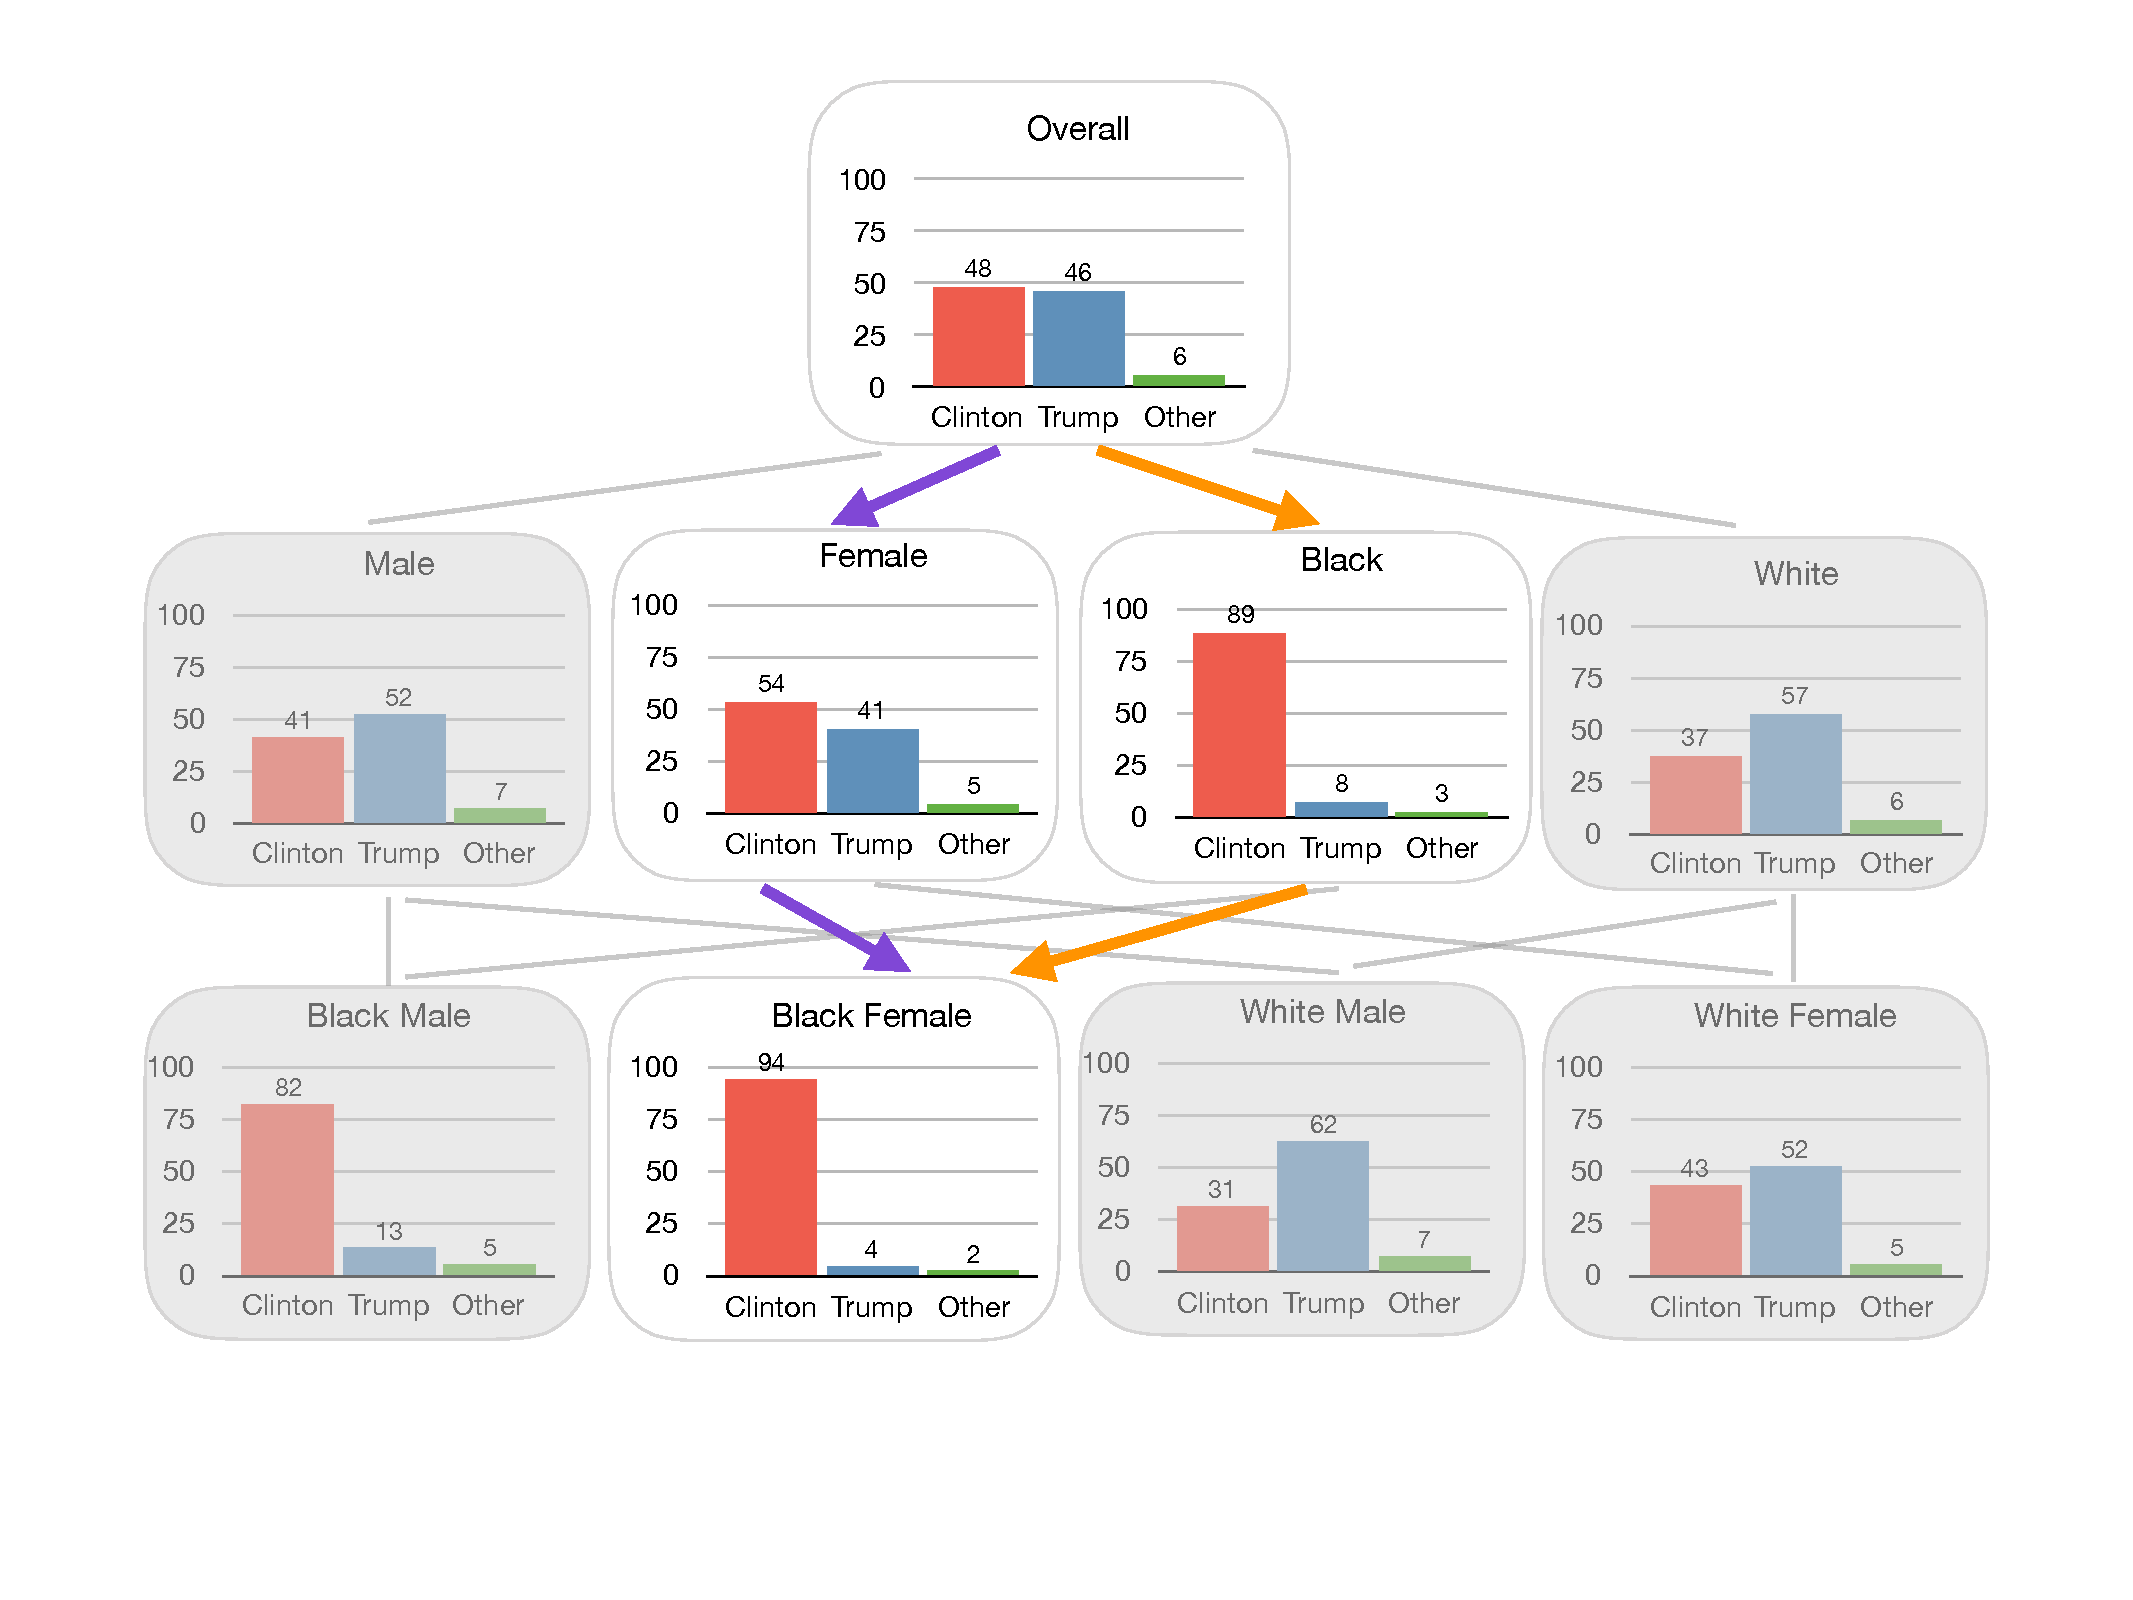
\includegraphics[width=\linewidth]{figures/elections_example_lattice.pdf}
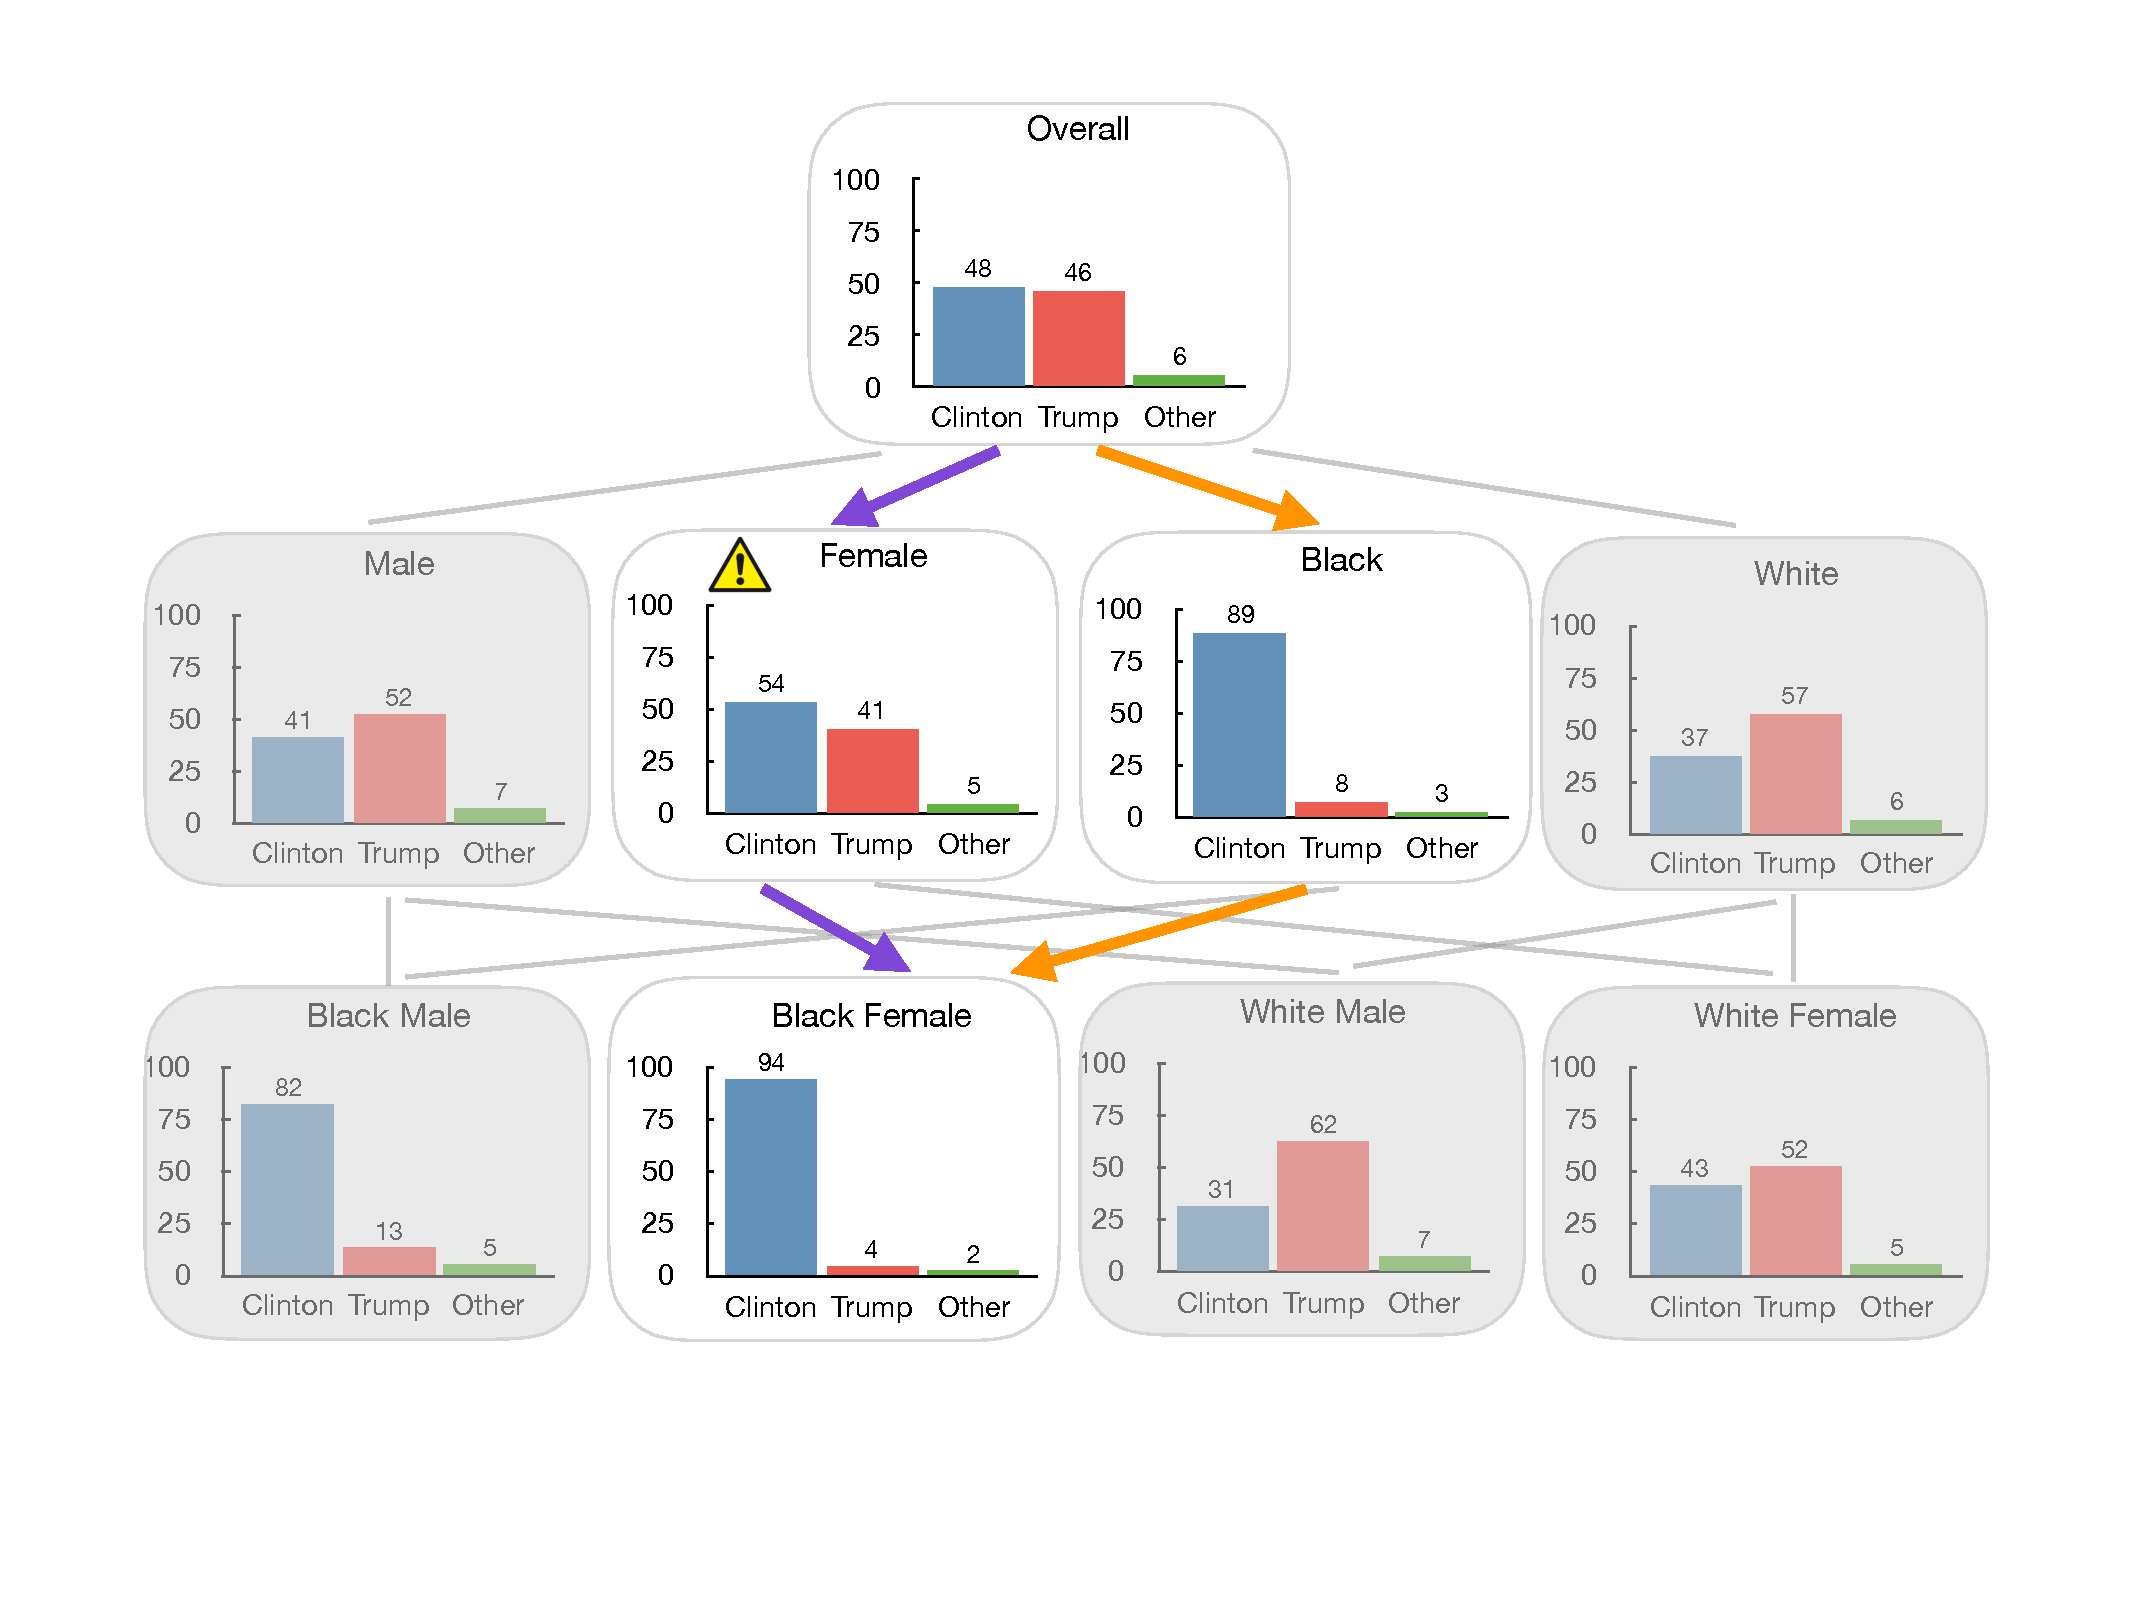
\includegraphics[width=\linewidth]{figures/elections_example_lattice_teaser.pdf}
\caption{Example data subset lattice illustrating the drill-down fallacy along the orange path as opposed to the informative purple path.}
\label{fig:elections_example}
\end{figure}

%Challenges associated with drill-down
There are three challenges associated with drilling down in this way. The first is that it is often not clear which attributes to drill-down on. Analysts may use their intuition for this, but this biased exploration may lead to large swaths of the lattice being ignored. The second challenge is that the path an analyst takes may lead to behavior that is not very surprising.  
For example, an analyst going from \texttt{Black} visualization to \texttt{Black Female} visualization in Figure 1 may find the two distribution to be similar, and therefore not surprising. This is in effect a wasted effort on the part of the analyst. The third challenge involves the \lq\lq drill-down fallacy\rq\rq . As shown in Figure~\ref{fig:elections_example}, an analyst can either arrive at the \texttt{Black Female} visualization by going through the purple or orange drill-down path. An analyst that followed the purple path may be surprised at how drastically the \texttt{Black Female} voting behavior differs from that of \texttt{Female}. This behavior is no longer surprising if the analyst had went down the orange path, where the proper reference (vote distribution for \texttt{Black}) explains the vote distribution for \texttt{Black Female}. That is, even though the vote distribution for 
\texttt{Black Female} is very different from that of \texttt{Female}, it can be explained by a more general phenomenon or \lq\lq root cause\rq\rq ---the vote distribution for \texttt{Black} community.

The aforementioned example demonstrates \emph{drill-down fallacy}---incomplete insights that result from potentially confounding factors not explored along a drill-down path. In particular, while performing a drill-down, an analyst may find a \lq\lq local difference\rq\rq\ in trends, without being aware of the more \lq\lq general phenomenon\rq\rq\ that could explain the trend of interest. This is because of the random selection of drill-down attribute. If an analyst randomly selects an attribute to drill down on, he may not come across the proper reference (visualization) that explains the behavior of the visualization of interest. Thus, they are at risk of falling prey to the drill-down fallacy. A naive solution to avoid this fallacy is to explore all potential pathways along the drill-down path. For example, generating and exploring visualizations for both race and gender based demographics, before exploring any of their combinations. Unfortunately, this approach does not scale with increasing number of factors in the drill-down path.

In this paper, we develop a visual data exploration tool that aims the three challenges: (iii) \textbf{Summarization.} collectively summarize the key insights from lattice, (ii) \textbf{Saliency.} capture globally insightful phenomena that satisfy safety criteria, and (iii) \textbf{Safety.} present proper (informative) reference for shown visualizations. Our tool automatically identifies the best possible drill-down paths that lead to \emph{informative insights}, and simulataneously summarizes the paths to form a hierarchy of visualizations. The challenge of building such tool includes considerations for how each visualization influences user's perception on other visualizations and selecting a set of visualization that are collectively interesting amongst a large set of visualization. To address this challenge, we develop a notion of \emph{informativeness}, defined as the capability of an reference visualizations to explain the visualization of interest. Informative visualizations helps users identify meaningful insights that arise from something \textit{actually interesting} about the data (instead of confounding variables), thereby preventing users from the drill-down fallacy. Our user study result demonstrates that our tool that make use of this notion of informativeness can guide an analyst towards meaningful insights. The contribution of this paper include:
\begin{denselist}
\item Introducing the novel concept of \emph{informativeness} that helps avoid drill-down fallacy in data exploration (Section 3),
\item Designing a tool that automatically identifies the best possible drill-down paths based on informative insights, and simultaneously summarizes those to form a unified perspective (Section 4),
\item Demonstrating the efficacy of our system through a comprehensive user study evaluation (Section 5).
\end{denselist}

\iffalse

%Exploring multidiemnsional dataset is hard.
Visual data exploration is the \emph{de facto} first step in understanding a multi-dimensional dataset. This exploration serves a variety of purposes: identifying trends and patterns, spotting outliers and anomalies, and verifying hypotheses. However, as datasets grow in size and complexity, visual data exploration unfolds several challenges for the analysts. For example, to identify patterns that merit further investigation, an analyst needs to explore different subsets of the data, which grows exponentially w.r.t. the number of attributes. Generating and examining visualizations for this combinatorial space of data subsets is a major bottleneck in the exploration process.

%Drill-Down for exploration
A common practice of analysts that escapes the combinatorial space is to perform selective drill-downs. Specifically, an analyst generates visualizations to gain an overview of the data, then drills down to interesting subsets to generate more visualizations. For example, a campaign manager may be interested in understanding the voting patterns across different demographics (say, race, gender, social class) using the 2016 US election exit polls\footnote{https://edition.cnn.com/election/2016/results/exit-polls}. A natural first step would be to generate a bar chart for the entire population, where the x-axis shows the election candidates and the y-axis the percentage of votes for each of these candidates. They can then drill down to specific demographics of interest, say gender-based demographics, by generating bar charts for female voters.

\begin{figure}[h!]
% 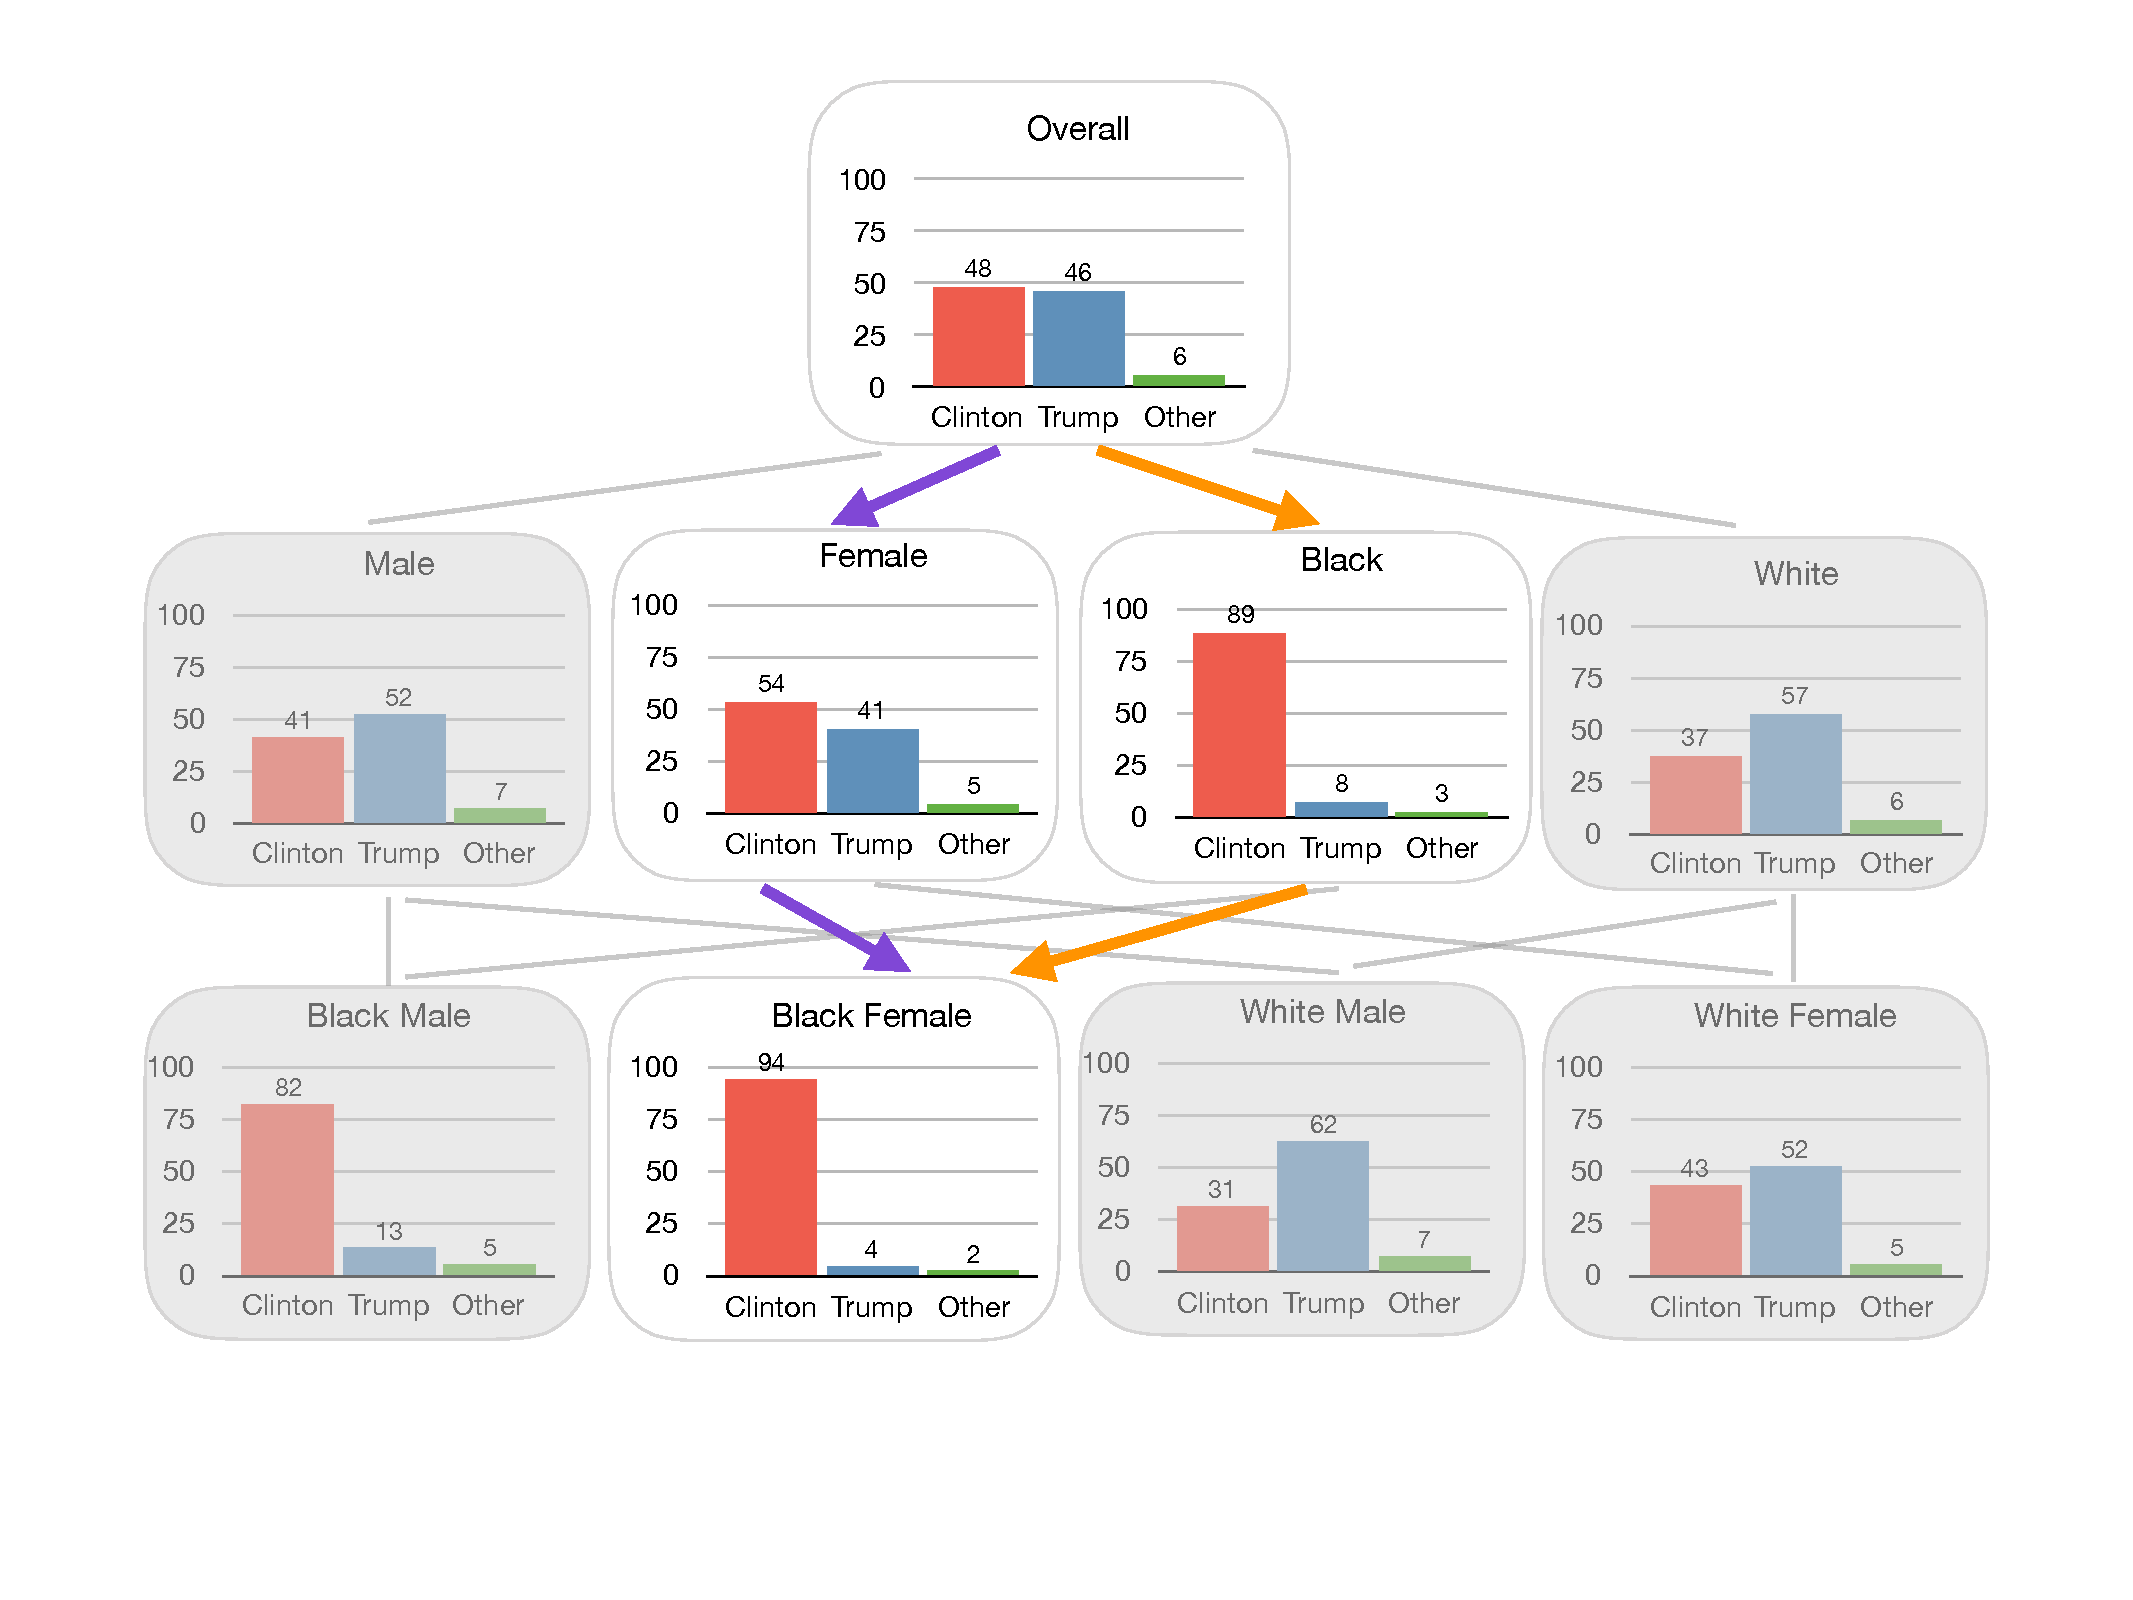
\includegraphics[width=\linewidth]{figures/elections_example_lattice.pdf}
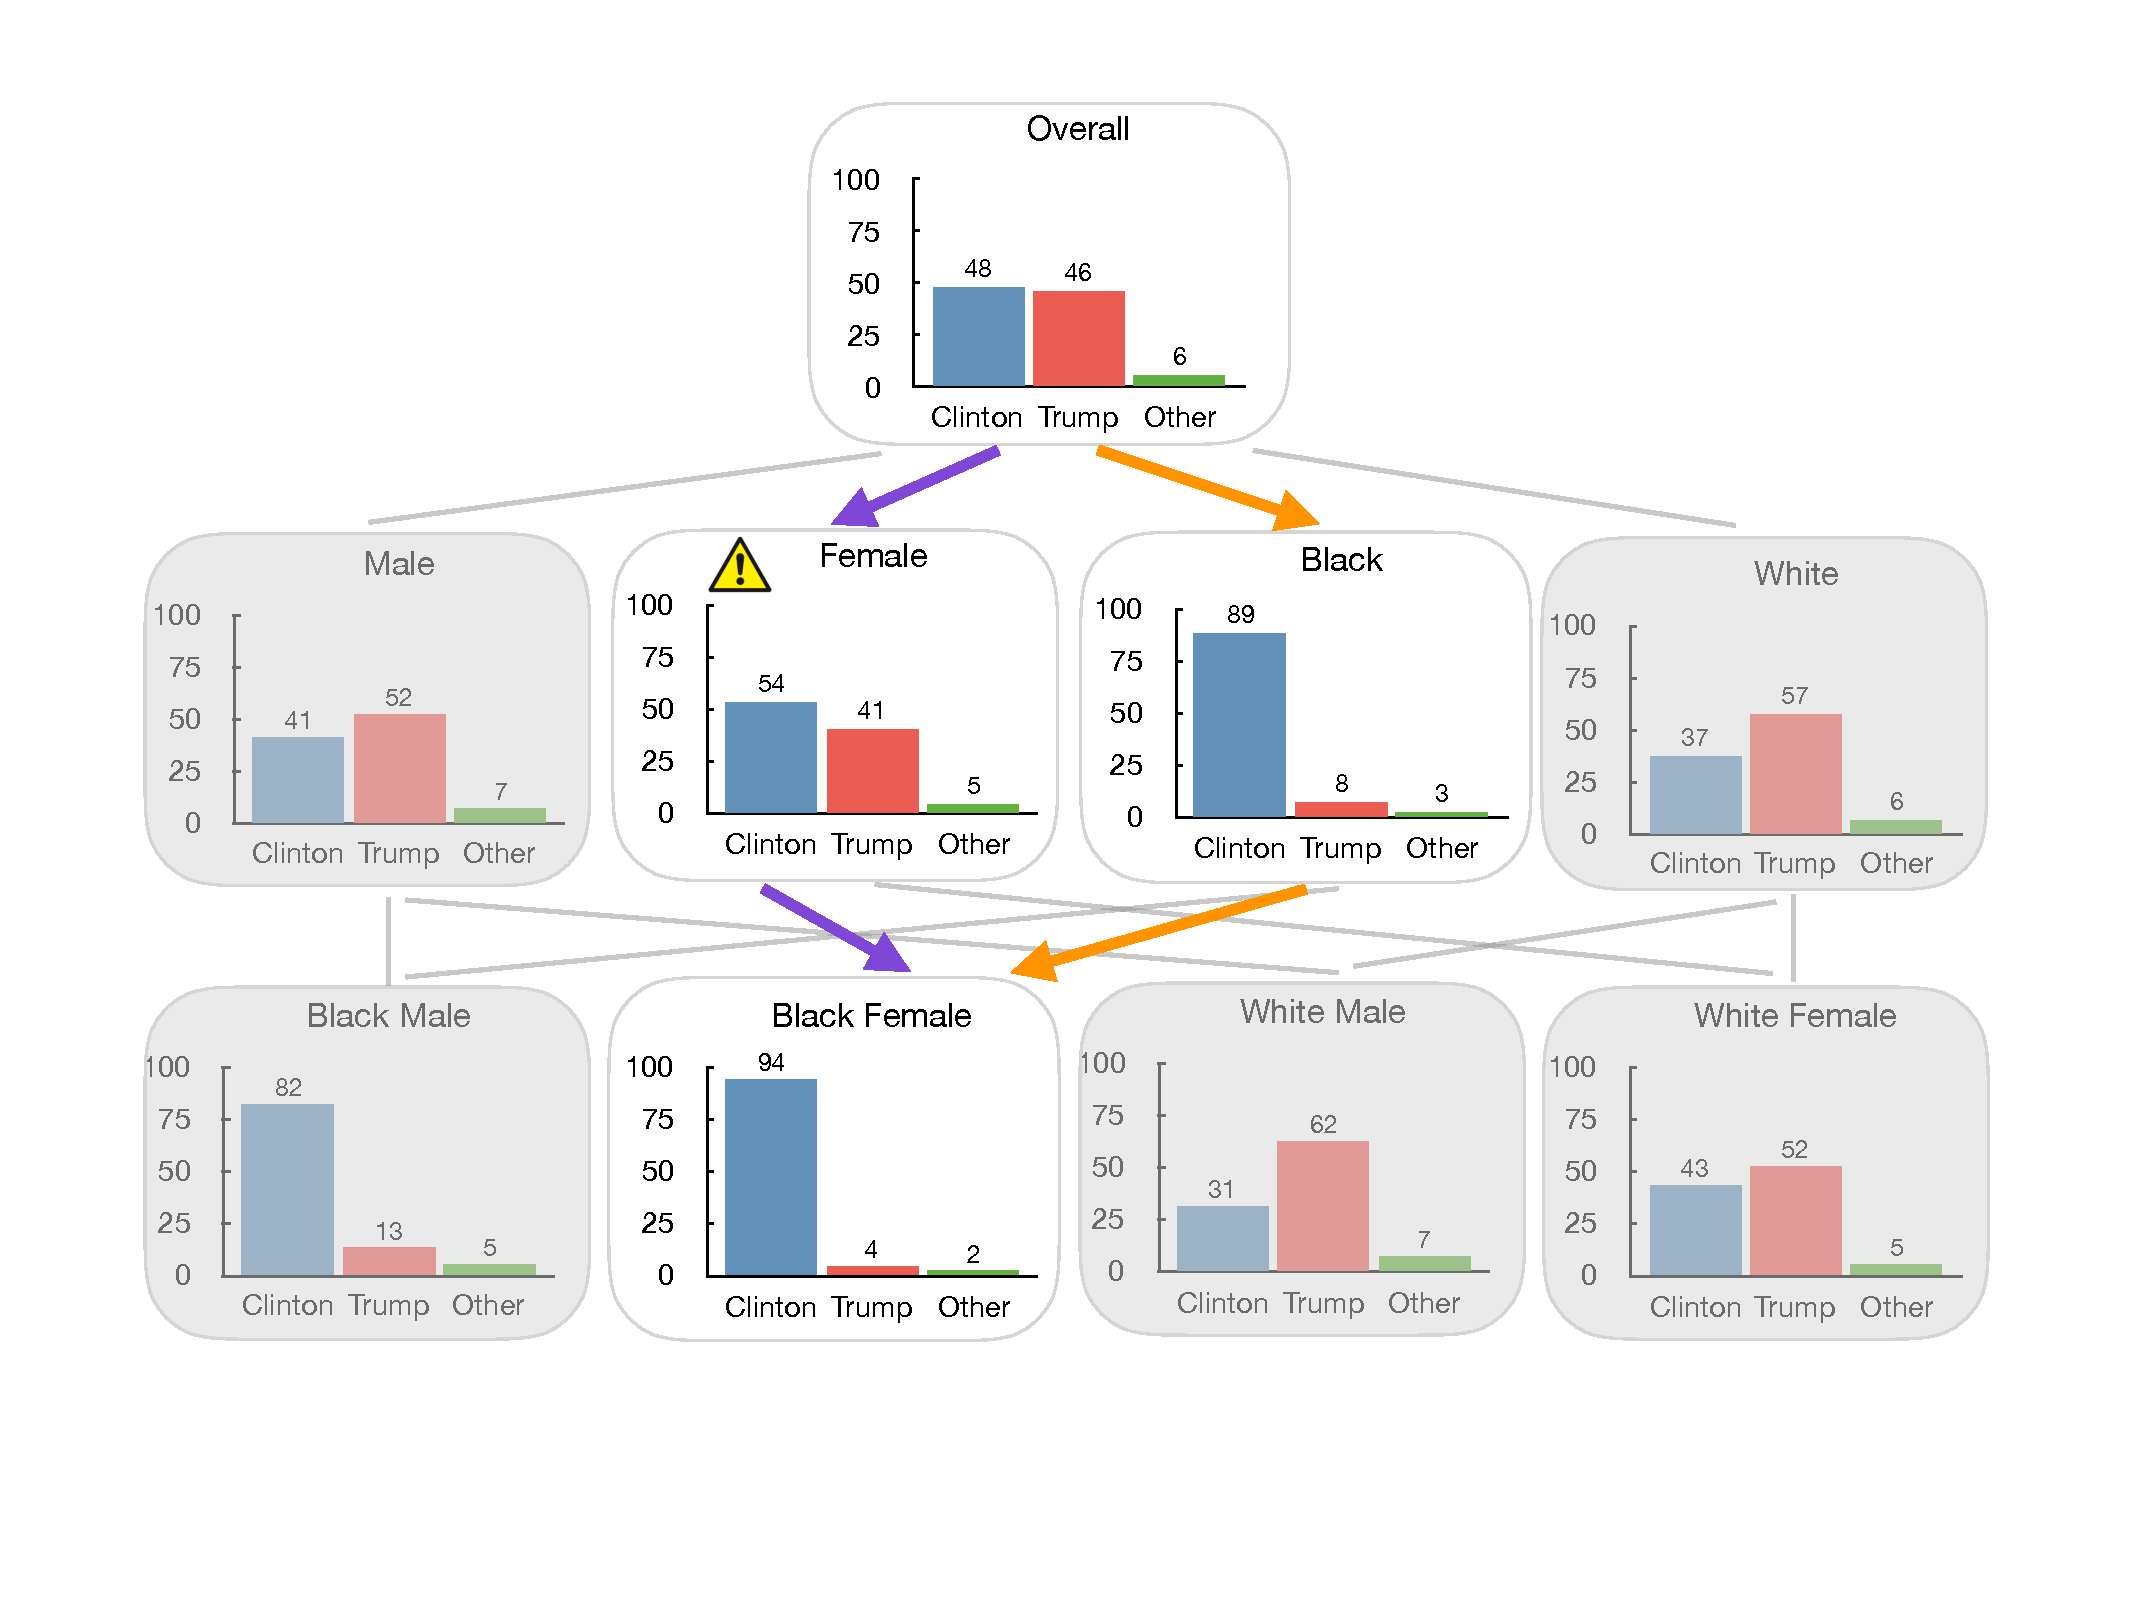
\includegraphics[width=\linewidth]{figures/elections_example_lattice_teaser.pdf}
\caption{Example data subset lattice illustrating the misleading factor fallacy along the orange path as opposed to the informative purple path.}
\label{fig:elections_example}
\end{figure}

%Drill-Down Fallacy

During this exploration process each drill-down may lead to insights, which derive from the observed visualizations. As shown in Figure~\ref{fig:elections_example}, an analyst can either arrive at the \texttt{Black Female} visualization by going through the purple or orange drill-down path. An analyst that followed the purple path may be surprised at how drastically the \texttt{Black Female} voting behavior differs from that of \texttt{Female}. This behavior is no longer surprising if the analyst had went down the orange path, where the proper reference (vote distribution for \texttt{Black}) explains the vote distribution for \texttt{Black Female}. That is, even though the vote distribution for 
\texttt{Black Female} is very different from that of \texttt{Female}, it can be explained by a more general phenomenon or \lq\lq root cause\rq\rq ---the vote distribution for \texttt{Black} community.

The aforementioned example demonstrates \emph{drill-down fallacy}---incomplete insights that result from potentially confounding factors not explored along a drill-down path. In particular, while performing a drill-down, an analyst may find a \lq\lq local difference\rq\rq\ in trends, without being aware of the more \lq\lq general phenomenon\rq\rq\ that could explain the trend of interest. This is because of the random selection of drill-down attribute. If an analyst randomly selects an attribute to drill down on, he may not come across the proper reference (visualization) that explains the behavior of the visualization of interest. Thus, they are at risk of falling prey to the drill-down fallacy. A naive solution to avoid this fallacy is to explore all potential pathways along the drill-down path. For example, generating and exploring visualizations for both race and gender based demographics, before exploring any of their combinations. Unfortunately, this approach does not scale with increasing number of factors in the drill-down path.

In this paper, we develop a visual data exploration tool with three-fold objectives: (i) \textbf{Safety.} present proper (informative) reference for shown visualizations, (ii) \textbf{Saliency.} capture globally insightful phenomena that satisfy our safety criteria, and (iii) \textbf{Summarization.} present a connected (unified) perspective. Our tool automatically identifies the best possible drill-down paths that lead to \emph{informative insights}, and simulataneously summarizes the paths to form a hierarchy of visualizations. The challenge of building such tool includes considerations for how each visualization influences user's perception on other visualizations and selecting a set of visualization that are collectively interesting amongst a large set of visualization. To address this challenge, we develop a notion of \emph{informativeness}, defined as the capability of an reference visualizations to explain the visualization of interest. Informative visualizations helps users identify meaningful insights that arise from something \textit{actually interesting} about the data (instead of confounding variables), thereby preventing users from the drill-down fallacy. Our user study result demonstrates that our tool that make use of this notion of informativeness can guide an analyst towards meaningful insights. The contribution of this paper include:
\begin{denselist}
\item Introducing the novel concept of \emph{informativeness} that helps avoid drill-down fallacy in data exploration (Section 3),
\item Designing a tool that automatically identifies the best possible drill-down paths based on informative insights, and simultaneously summarizes those to form a unified perspective (Section 4),
\item Demonstrating the efficacy of our system through a comprehensive user study evaluation (Section 5).
\end{denselist}

To understand a multi-dimensional dataset, analysts often apply OLAP (Online Analytical Processing) operators to explore the space of attributes~\cite{Gray1997}. A common OLAP task includes generating visualizations to gain an overview of the data, then drilling down to interesting subsets to generate more visualizations. For example, a campaign manager may be interested in understanding the voting patterns across different demographics (say, race, gender, social class) using the 2016 US election exit polls\footnote{https://edition.cnn.com/election/2016/results/exit-polls}. A natural first step is to generate a bar chart for the entire population, where x-axis shows the election candidates and y-axis the percentage of votes for these candidates. He can then drill down to specific demographics of interest, say gender-based demographics by generating bar charts for female voters. %A further drill-down on race will lead to more specific demographics such as white male, and black female. 
\begin{figure}[h!]
% 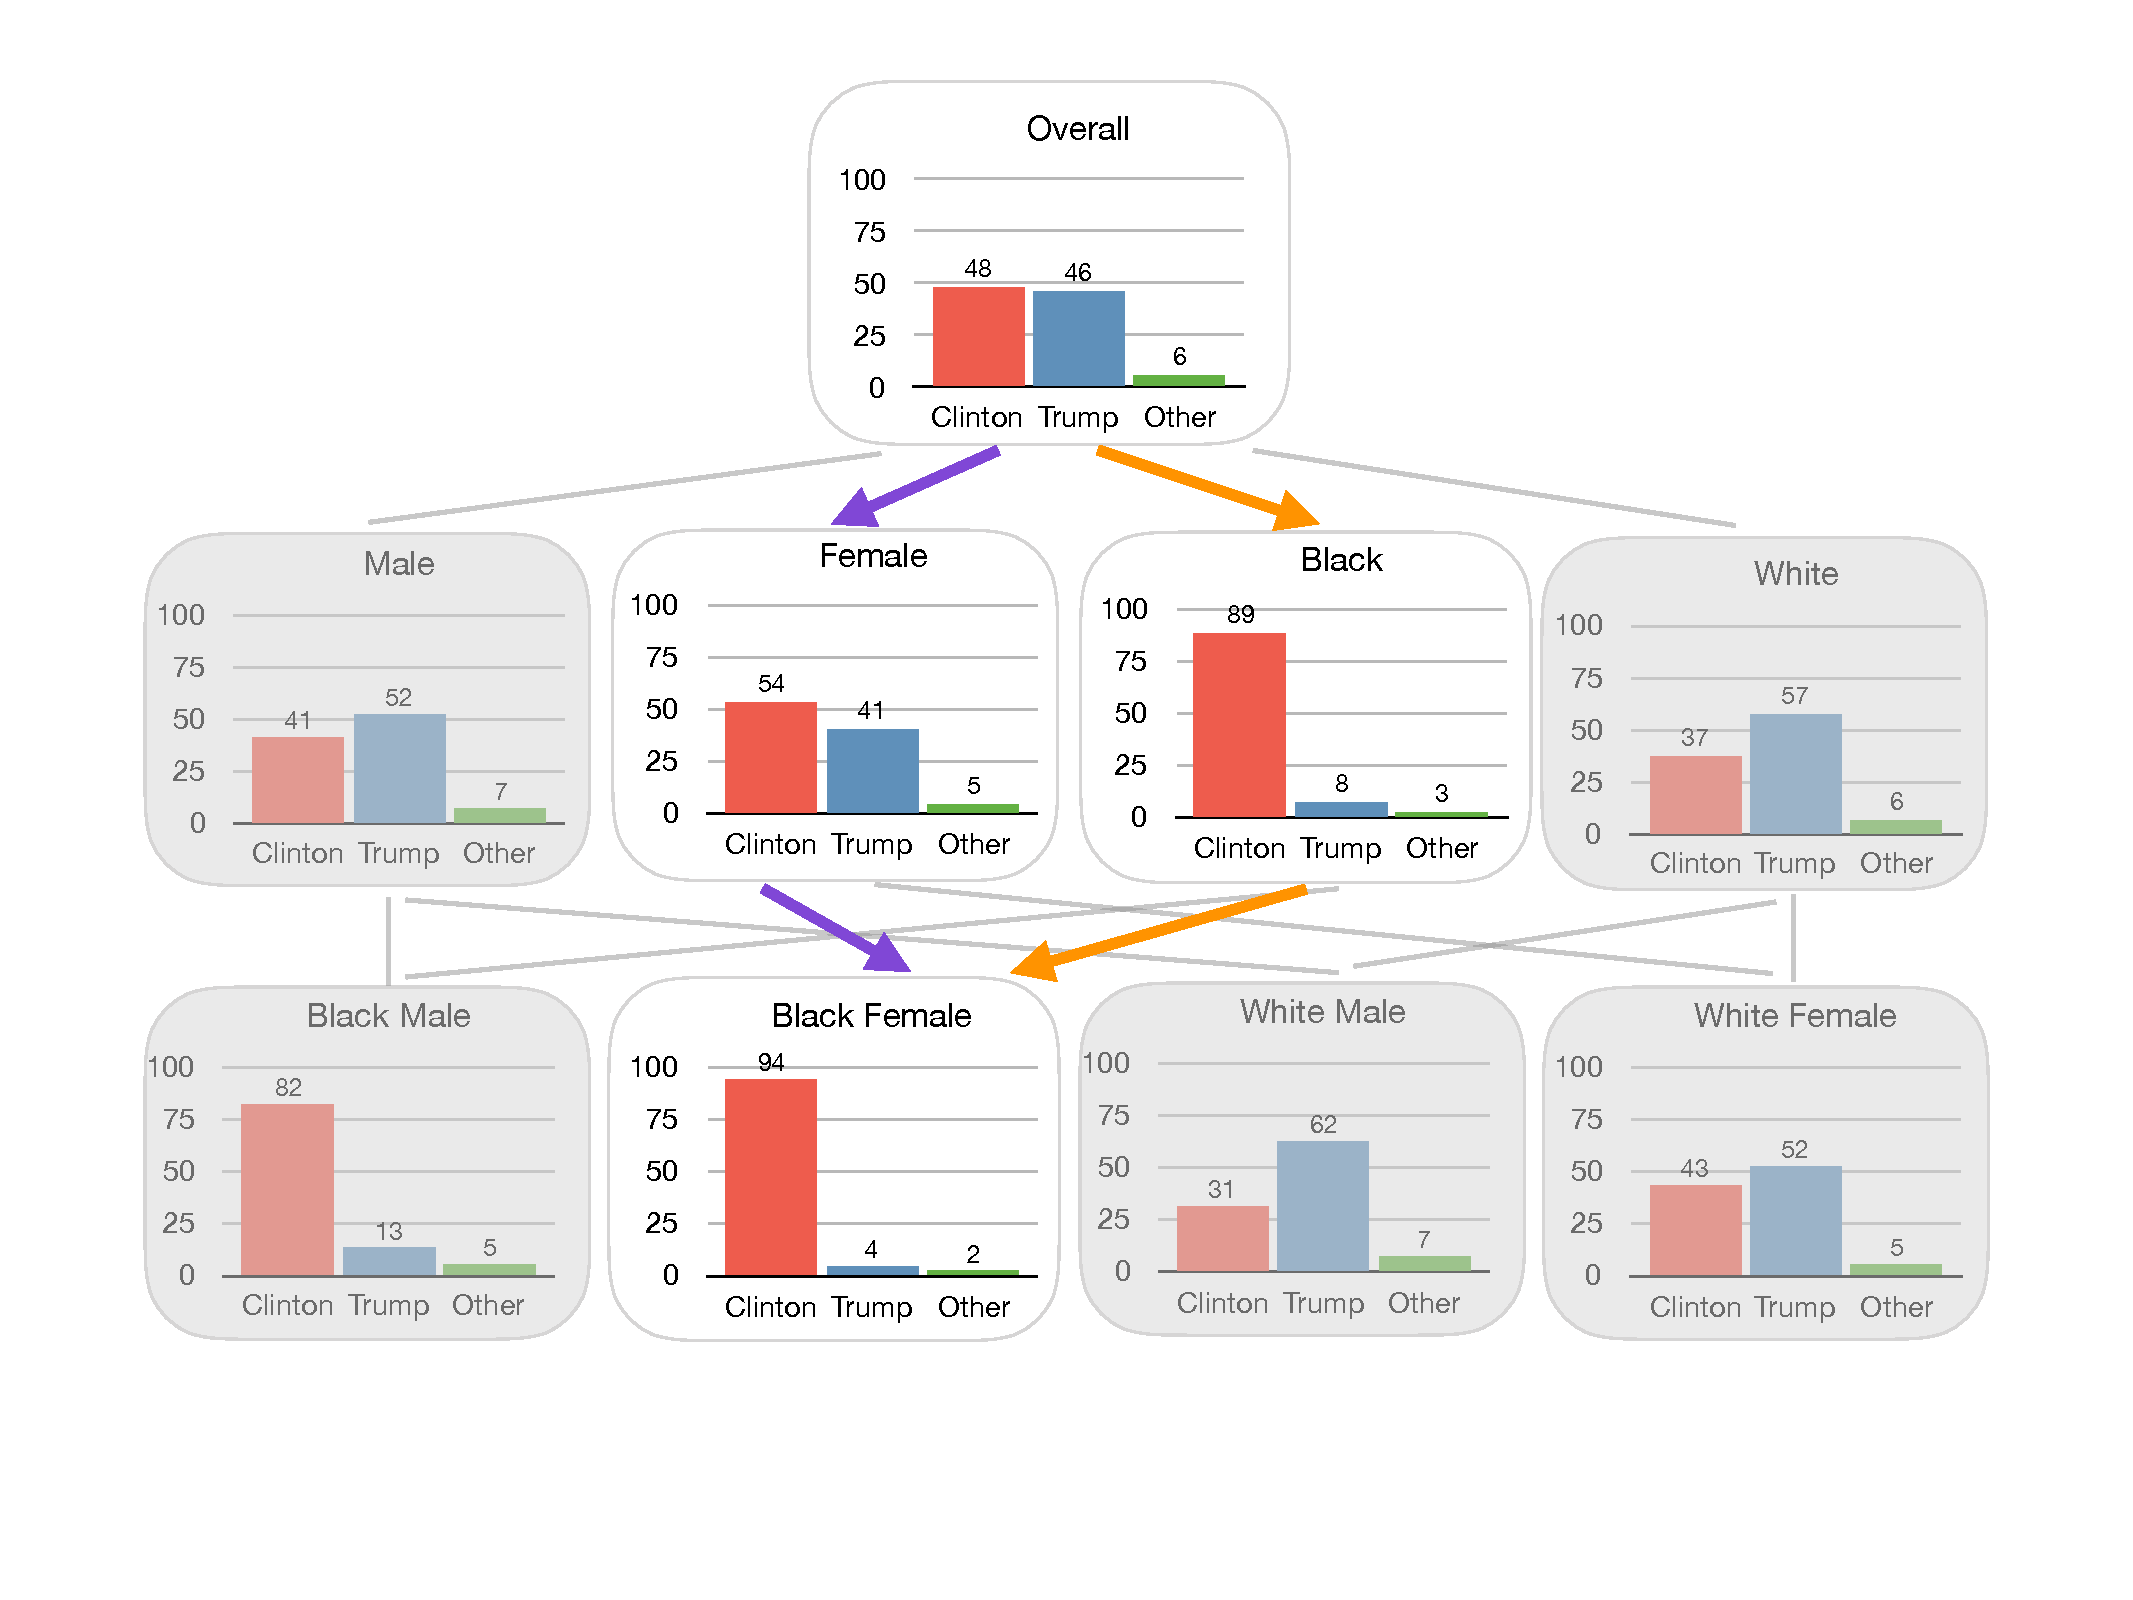
\includegraphics[width=\linewidth]{figures/elections_example_lattice.pdf}
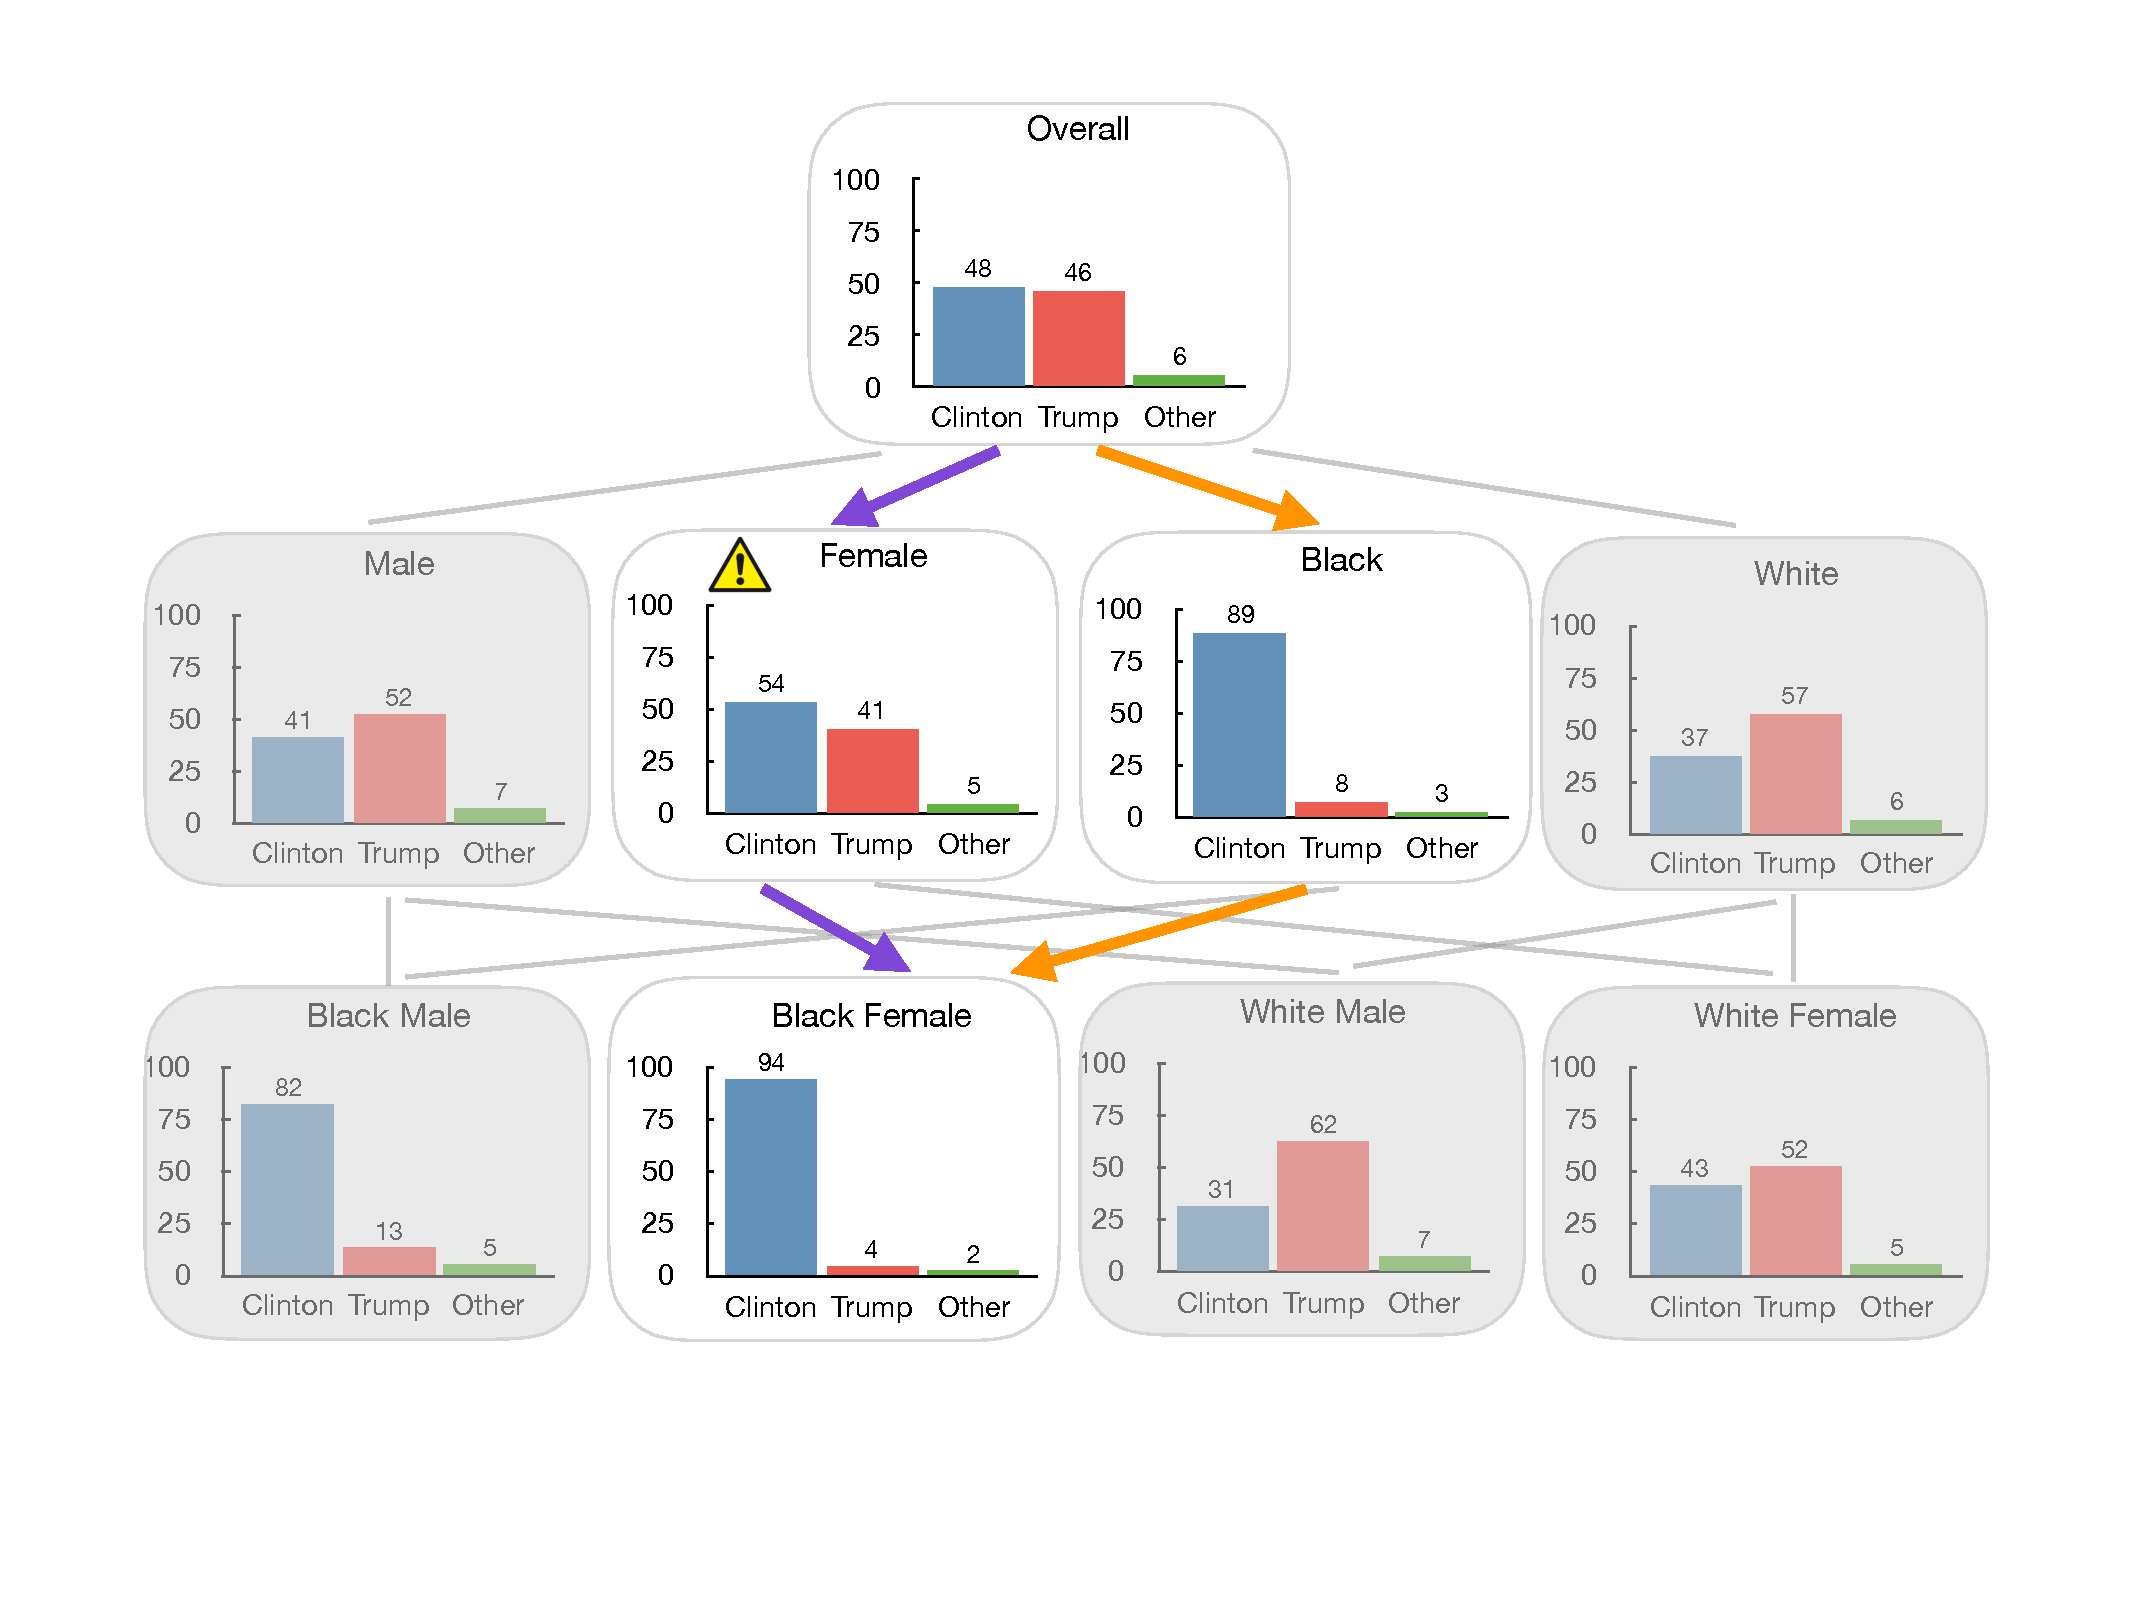
\includegraphics[width=\linewidth]{figures/elections_example_lattice_teaser.pdf}
\caption{Example data subset lattice illustrating the misleading factor fallacy along the orange path as opposed to the informative purple path.}
\label{fig:elections_example}
\end{figure}
In this exploration process each drill-down may lead to insights, which derive from the observed visualizations. As shown in Figure~\ref{fig:elections_example}, an analyst can either arrive at the Black Females visualization by going through the purple or orange drill-down path. At random, an analyst that followed the purple path may be surprised at how drastically the Black Female voting behavior differs from the vote distribution for females. This behavior is no longer surprising if the analyst had went down the orange path, where the proper reference (vote distribution for Black) explains the behavior of the Black Female distribution. The misleading insight is a result of the order in which the drill-down has been performed. This example demonstrates a case of \emph{drill-down fallacy}, which results from potentially confounding factors not explored along a drill-down path.

% For example, the drill-down on gender shows that the female voting pattern follow the trend of overall population, whereas a further drill-down on race shows that the trend of black females differ from that of females. Many existing tools will flag the latter as a potential insight, since the black females exhibit a high deviation with respect to an observed parent. The insight, however, is a by-product of the order in which the drill-down has been performed---drilling down on race before gender will explain the trend of black females in light of black demographic. 

When an analyst explore a dataset by randomly selecting the attribute to drill down on, they may not come across the proper reference visualization that explains the behavior of the visualization of interest. Thus, they are at risk of falling prey to the drill-down fallacy. A naive solution to avoid this fallacy is to explore all potential pathways along the drill-down path. For example, generating and exploring visualizations for both race and gender based demographics, before exploring any of their combinations. Unfortunately, this approach does not scale with increasing number of factors in the drill-down path.

In this paper, we develop a tool to help users explore a dataset while avoiding improper references that may lead to drill-down fallacy. Our tool automatically identifies the best possible drill-down paths that lead to \emph{informative insights}, and summarizes the paths. The challenge of building such tool includes considerations for how each visualization influences user's perception on other visualizations and selecting a set of visualization that are collectively interesting amongst a large set of visualization. To address this challenge, we develop a notion of \emph{informativeness}, defined as the capability of an reference visualizations to explain the visualization of interest. Informative visualizations helps users identify meaningful insights that arise from something \textit{actually interesting} about the data (instead of confounding variables), thereby preventing users from the drill-down fallacy. Our user study result demonstrates that our tool that make use of this notion of informativeness can guide an analyst towards meaningful insights. The contribution of this paper include:
\begin{denselist}
\item Introducing the novel concept of \emph{informativeness} that helps avoid drill-down fallacy in data exploration (Section 3),
\item Designing a tool that automatically identifies the best possible drill-down paths based on informative insights, and summarizes those (Section 4),
\item Demonstrating the efficacy of our system through a comprehensive user study evaluation (Section 5).
\end{denselist}

%\par Common analytics tasks, such as causal inference, feature selection, and outlier detection require studying data distributions at different levels of data granularity~\cite{Anand2015,Wu2013,Heer2012}. For example, a campaign manager may be interested in the voting patterns across different demographics (say, race, gender, social class) using the 2016 US election exit polls\footnote{\url{https://edition.cnn.com/election/2016/results/exit-polls}} to identify demographic groups for targeted advertisement. Visual analysis is the common approach for performing such analytics tasks, in which an analyst constructs visualizations to capture the distributions at different subsets of data. The goal of this visual analysis is to extract meaningful insights---when a set of visualizations along with human interpretation leads to informative and interesting facts about the underlying distributions.

%\par However, without knowing \textit{what} subset of data contains an insightful distribution, manually exploring distributions from all possible data subsets can be tedious and inefficient. For example, the aforementioned campaign manager could construct bar charts for all possible demographics, where x-axis shows the election candidates and y-axis the percentage of votes for these candidates. Subsequently, he may visually compare these bar charts to understand how voting pattern changes across different demographics. Even after constructing the visualizations for all possible data subsets, which itself is a daunting task, currently there is no systematic way for the campaign manager to make sense of or even navigate through this large space of possible visualizations to draw meaningful insights. %Both exercises, first, constructing the large number of visualizations corresponding to all possible data subsets, and then, navigating through this large space of visualizations to draw meaningful insights is challenging, particularly because there is no systematic way to perform these exercises.

%\par To this end, we present \system, an interactive visualization summarization system that automatically selects a small set of visualizations to summarize the distributions within a dataset in an informative manner. Our system is motivated by our observation that when an analyst is aware of the distributions present in different data subsets, she can draw meaningful insights and establish correlations about related visualizations that she has not yet seen with ease. We define this aspect of dataset understanding as \emph{distribution awareness}. For example, based on the vote distributions for different demographics shown in Figure~\ref{fig:elections_example}, an analyst can infer that most demographic groups have similar voting behaviors for `Clinton' and `Trump' (a,b,c,e,f), whereas black demographic groups are strongly skewed towards voting for `Clinton' (d,g,h). Since human analysts have limited time and memory, it is often impossible to explore visualizations from all data subsets. An ideal summarization system should display visualizations that enables the analyst to achieve \emph{maximal distribution awareness}, from which she can reasonably approximate most of the remaining unseen visualizations in a dataset.

%\par Nevertheless, finding effective visualizations to summarize a dataset is not as trivial as picking individual visualizations that maximizes some statistical measure, such as deviation~\cite{Vartak2015}, coverage~\cite{Sarvghad2017}, or significance testing~\cite{Anand2015}, which can often result in misleading summarizations. For example, if the campaign manager uses a deviation based metric to identify insightful distributions \cite{Vartak2015}, he could find that the voting pattern of black females is drastically different from the voting pattern of general female population. Accordingly, he might allocate his advertisement funds to target the black female population. While black females do defy the trends of general females, the comparison is incomplete, since it ignores the fact that black females very closely follows the voting pattern of the black population. Accordingly, the proper demographic to target should be the black population rather than the more specific black female population.

%Consider an elections campaign manager who is allocating the advertisement budget to be spent on different demographic populations to target for an upcoming election by investigating the voting patterns across different demographic groups. He performs a randomized permutation testing between the gender and race attributes and finds that the voting pattern of black females is drastically different from the voting pattern of general female population and allocates the his advertisement funds to target the black female population. While black females do defy the trends of general females, the comparison is incomplete, since it ignores the fact that black females follows very closely to the distribution of the voting behavior of the black population, so the proper subpopulation to target should be the black population rather than the more specific black female population.

%Even after constructing the visualizations for all possible data subsets, which itself is a daunting task, currently there is no systematic way for our campaign manager to make sense of or even navigate through this large space of possible visualizations to draw meaningful insights.

%\par The goal of visual analysis is to extract meaningful stories or insights from the data. Individual visualizations represent simple ``factoids'' portraying one aspect of the data. Meaningful insights arise when a group of factoids work in conjunction, along with human interpretation, to produce informative and interesting facts.
%\par However, without knowing \textit{what} subset of the data would be interesting to visualize, manual drill-downs and roll-ups on all possible filter combinations can be tedious and inefficient for analysts. In many data analytics scenarios, analysts have an x and y axis of interest and want to explore data subsets corresponding to different filtering criteria. For example, a campaign manager may be interested in looking at bar chart visualizations of x as the voted candidate and y as the percentage of votes for the 2016 US elections exit polls with different filter combinations on demographics information, such as gender, income, race, states, and responses to different survey questions\footnote{\url{https://edition.cnn.com/election/2016/results/exit-polls}}. The analyst would have to compare across a combinatorially large space of different data subsets by iteratively changing the filter criterion of a visualization to understand how the relationship between the x and y variables change across data subsets. Even if the analyst had plotted visualizations for all possible data subsets, currently there is no systematic and effective way for an analyst to make sense of and navigate through the large space of possible visualizations to draw meaningful insights.
%\par To this end, we present \system, an interactive visualization summarization system that automatically selects a small set of visualizations to summarize the data distributions within a dataset in an informative manner. When analysts inspect informative visualizations that cover these insights, they associate particular sets of attributes to typical trends and observed patterns. We define this aspect of dataset understanding as \emph{distribution awareness}. For example, we observe that in Figure~\ref{fig:elections_example}, most of the visualizations has `Clinton' and `Trump' as comparably-sized bars with `Others' being a small fraction of the overall (a,b,c,e,f), whereas visualizations involving the Black population is highly skewed towards `Clinton' (d,g,h). Since human analysts have limited memory and attention, it is often impossible to visualize all possible data subsets. An ideal summarization system should display visualizations that enables users to gain maximal distribution awareness of the typical trends within a dataset.
%\par However, finding effective visualizations to summarize a dataset is not as trivial as picking individual visualizations that maximizes some statistical measure, such as deviation~\cite{Vartak2015}, coverage~\cite{Sarvghad2017}, or significance testing~\cite{Anand2015}, which can often result in misleading summarizations. Consider an elections campaign manager who is allocating the advertisement budget to be spent on different demographic populations to target for an upcoming election by investigating the voting patterns across different demographic groups. He performs a randomized permutation testing between the gender and race attributes and finds that the voting pattern of black females is drastically different from the voting pattern of general female population and allocates the his advertisement funds to target the black female population. \dor{Himel, can you check if this example makes sense? or should we say chi2? chi2 just give you columnar correlation info not at the attribute-level info? although probably only a deviation based comparison can give you a comparison like this.} While black females do defy the trends of general females, the comparison is incomplete, since it ignores the fact that black females follows very closely to the distribution of the voting behavior of the black population, so the proper subpopulation to target should be the black population rather than the more specific black female population.

The above example demonstrates a scenario where the selection of an improper reference (female) for comparing the visualization (black female) against results in misleading insights. In \system, we formulate an objective where a visualization is \emph{actually} interesting when it deviates from and can not be explained by \emph{even} its most informative reference. %\dor{can we add an example here?}
Our user study results described in Section~\ref{sec:userstudy} shows that this notion of informative interestingness can guide an analyst towards more meaningful stories for further investigation. The contribution of this paper include:
\begin{denselist}
\item Proposing the novel problem of visualization summarization and use cases highlighting the importance of \textit{distribution awareness} in dataset understanding (Section~\ref{sec:distributionaware}), %inform  visualization understanding and analytical tool designs
\item Formulating the structure and utility of the visualization search space (\emph{lattice}) using a user expectation model motivated by our formative study (Section~\ref{sec:datamodel}),
\item Designing efficient algorithms and optimizations to identify a set of informatively connected interesting visualizations (Section~\ref{sec:system}),
\item Presenting an interactive visualization dashboard interface that adopts a simple and intuitive hierarchical lattice layout (Section~\ref{sec:interaction}),
\item Demonstrate the efficacy of our system through a user study evaluation (Section~\ref{sec:userstudy}).
\end{denselist}
\fi

%\hdev{Let's take a step back, and look at the current flow in introduction. In the first paragraph, we vaguely motivate what can be considered as collective insights. In second paragraph, we try to connect the idea of collective insights with the challenges of data subset exploration. In third paragraph, we introduce two concepts: visual summarization, and distribution awareness. We do not clearly state what these two means. There's an example that conveys what could be captured through pattern or trend mining. In the fourth paragraph, we present an example to convey some specific challenges of visual summarization. The fifth paragraph states our contributions. My suggestion is to immediately jump into business by saying what we mean by distribution awareness, why is it important, and why is this challenging. We have the contents lying around already, it's just a matter of clearly stating these three aspects, preferably without using new abstractions.}
